\documentclass[tikz,border=2]{standalone}
\usetikzlibrary{shadows,decorations.pathreplacing,arrows,shapes,positioning,calc,backgrounds,fit}
\newcommand{\vanish}[1]{}
\usepackage{colortbl}
\usepackage{array}
\usepackage{amssymb}
\usepackage{multirow}
\newcommand{\shaded}[1]{\cellcolor{black!20}{#1}}
\newcommand{\calc}[1]{\mbox{$\mathcal{C}_{#1}$}}
\pdfpageattr {/Group << /S /Transparency /I true /CS /DeviceRGB>>}
\newcommand{\mathtttt}{}
% Define the layers to draw the diagram
%
\begin{document}
%% \pgfdeclarelayer{bg}
%% \pgfdeclarelayer{fg}
%% \pgfsetlayers{bg,main,fg}
\newcommand{\ttbig}{\mathtt{big}}
\newcommand{\ttsmall}{\mathtt{small}}
\newcommand{\ttwifi}{\mathtt{wifi}}
\newcommand{\ttcab}{\mathtt{cab}}
%
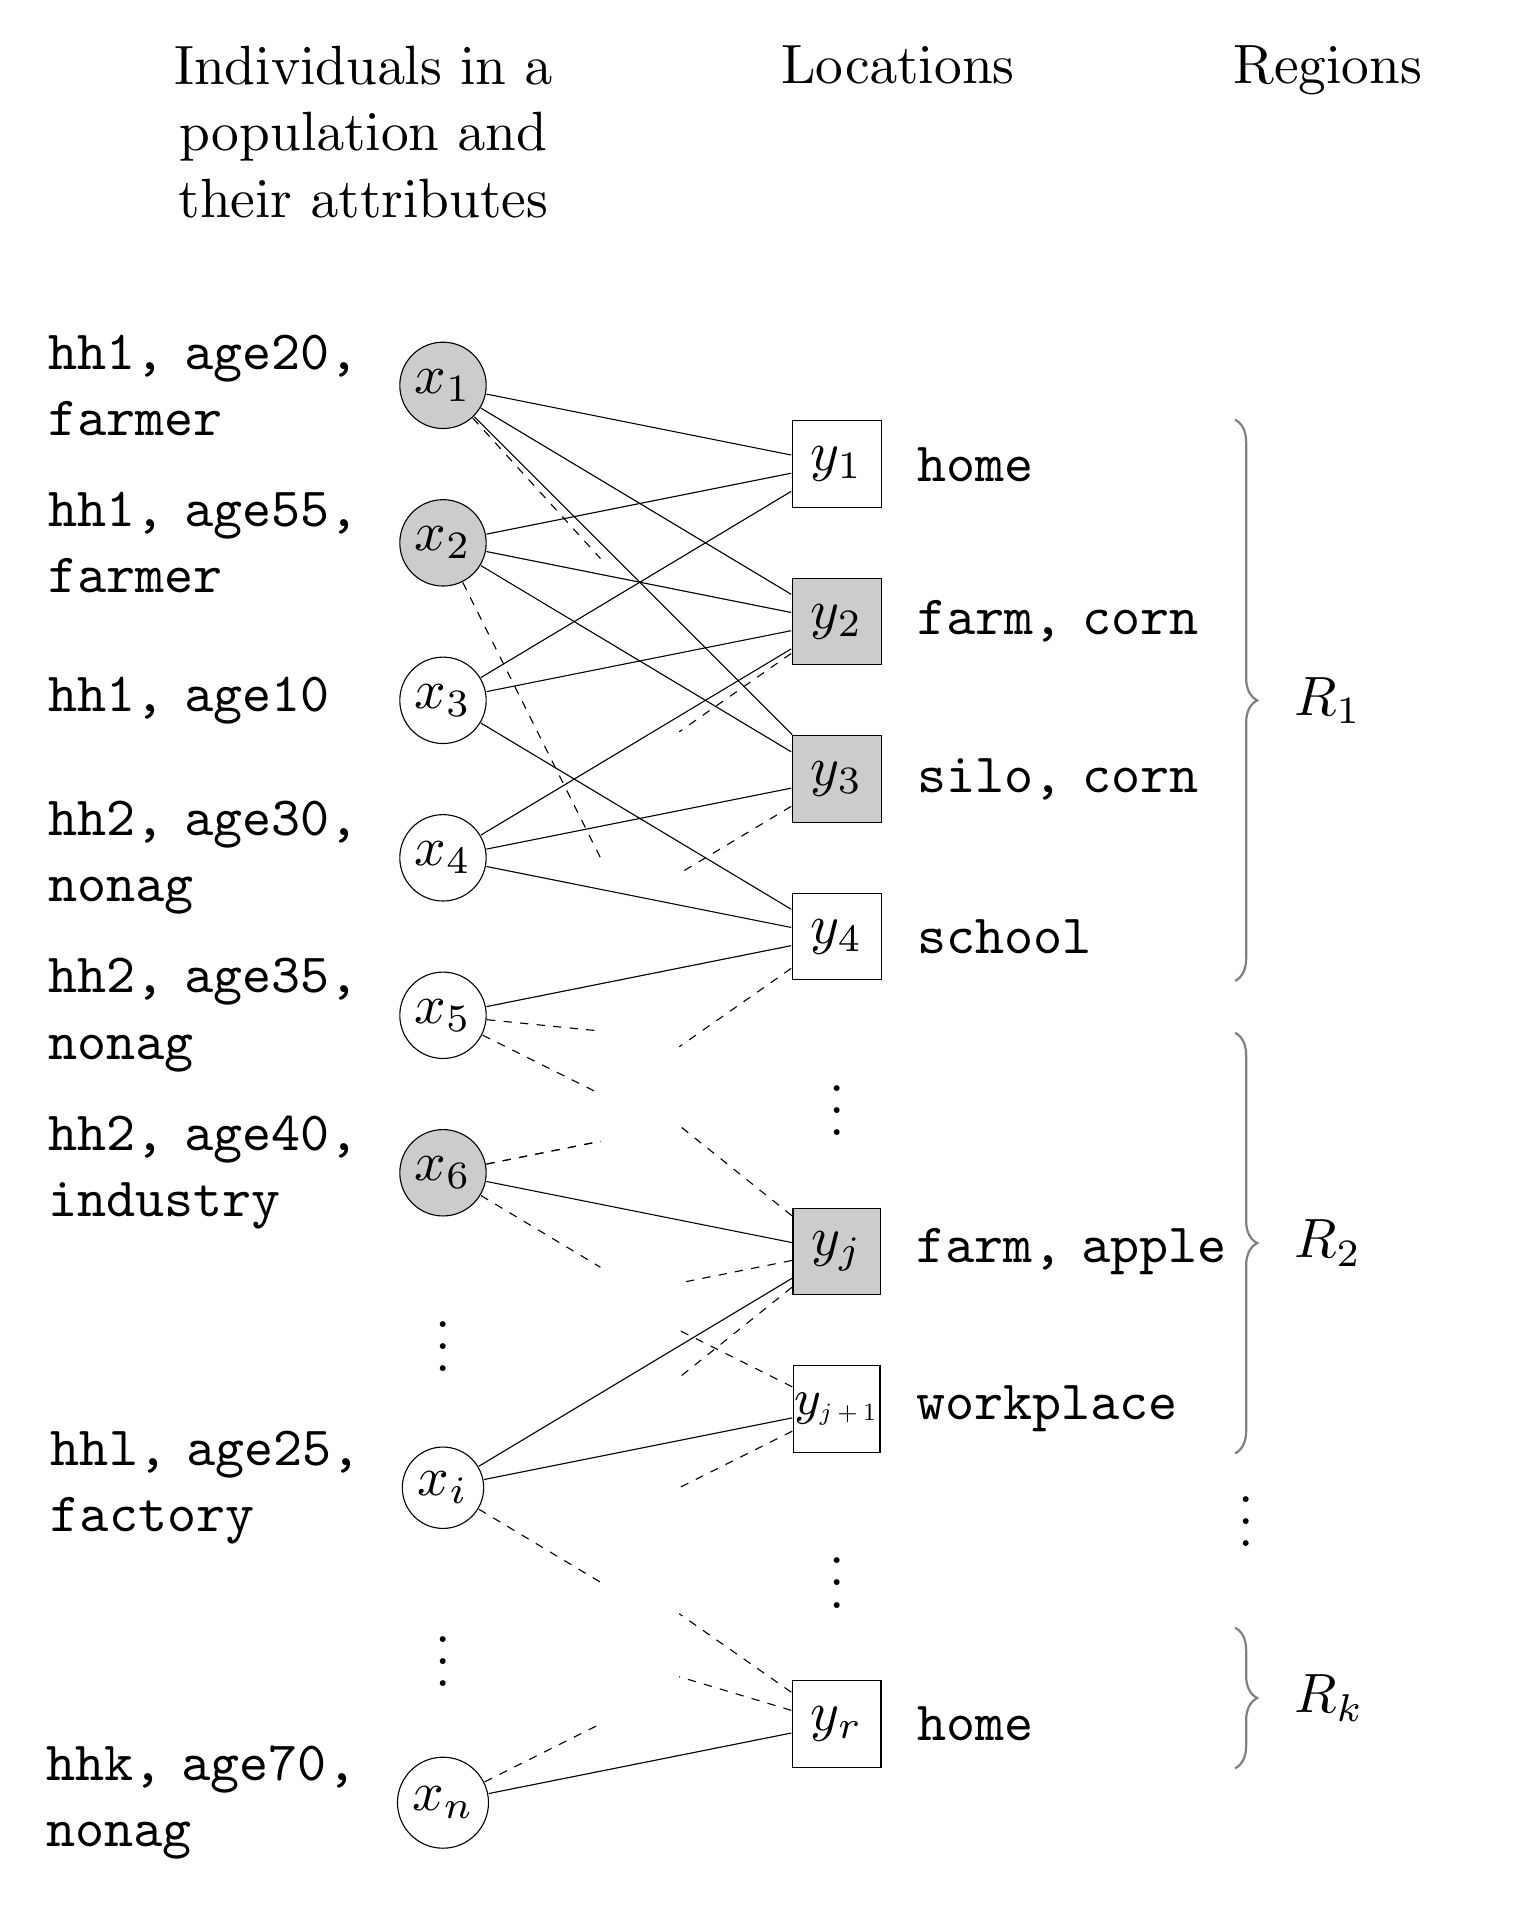
\begin{tikzpicture}
[scale=2,node distance=.5cm, transform shape,
    mybrace/.style={gray,decorate,decoration={brace,mirror,amplitude=8pt,raise=-4pt},yshift=0pt,thick},
    ag/.style={fill=black!20},
    agent/.style={draw,shape=circle,inner sep=.5mm},
    loc/.style={shape=rectangle,draw,minimum height=5.5mm,minimum
    width=5.5mm},
    lab/.style={fill=white,font=\scriptsize,inner sep=.5pt},
    prop/.style={text width=2cm,font=\tt},
myedge/.style={>=latex', shorten >=.0pt, shorten <=.0pt,semithick}]
%%%%%%%%%%
\begin{scope}[shift={(-2,-2.6)}]
%% nodes
\node (x1) [agent,ag] at (0,0)  {$x_1$};
\node (x2) [agent,ag] at (0,-1) {$x_2$};
\node (x3) [agent] at (0,-2) {$x_3$};
\node (x4) [agent] at (0,-3) {$x_4$};
\node (x5) [agent] at (0,-4) {$x_5$};
\node (x6) [agent,ag] at (0,-5) {$x_6$};
\node at (0,-6) {$\vdots$};
\node (xi) [agent] at (0,-7) {$x_i$};
\node at (0,-8) {$\vdots$};
\node (xn) [agent] at (0,-9) {$x_n$};

\def\locx{2.5}
\node (y1) [loc] at (\locx,-0.5) {$y_1$};
\node (y2) [loc,ag] at (\locx,-1.5) {$y_2$};
\node (y3) [loc,ag] at (\locx,-2.5) {$y_3$};
\node (y4) [loc] at (\locx,-3.5) {$y_4$};
\node (v1) at (\locx,-4.5) {$\vdots$};
\node (yj) [loc,ag] at (\locx,-5.5) {$y_j$};
\node (yj1) [loc,inner sep=0] at (\locx,-6.5) {\small $y_{\scalebox{.5}{$j+1$}}$};
\node (v2) at (\locx,-7.5) {$\vdots$};
\node (yr) [loc] at (\locx,-8.5) {$y_r$};
%% agent preferences
\node (px1) [prop,left=of x1,shift={(.4,0)}] {hh1, age20, farmer};
\node (px2) [prop,left=of x2,shift={(.4,0)}] {hh1, age55, farmer};
\node (px3) [prop,left=of x3,shift={(.4,0)}] {hh1, age10};
\node (px4) [prop,left=of x4,shift={(.4,0)}] {hh2, age30, nonag};
\node (px5) [prop,left=of x5,shift={(.4,0)}] {hh2, age35, nonag};
\node (px6) [prop,left=of x6,shift={(.4,0)}] {hh2, age40, industry};
\node (pxi) [prop,left=of xi,shift={(.4,0)}] {hhl, age25, factory};
\node (pxn) [prop,left=of xn,shift={(.4,0)}] {hhk, age70, nonag};
\node (ph) at (px1.north west) [shift={(0,.5)}, text width=4.0cm,
anchor=south west,align=center] {Individuals
in a \\ population and \\ their attributes};
%% resource properties
\node (py1) [right=of y1,shift={(-.4,0)},prop] {home};
\node (py2) [right=of y2,shift={(-.4,0)},prop] {farm, corn};
\node (py3) [right=of y3,shift={(-.4,0)},prop] {silo, corn};
\node (py4) [right=of y4,shift={(-.4,0)},prop] {school};
\node (pyj) [right=of yj,shift={(-.4,0)},prop] {farm, apple};
\node (pyj1) [right=of yj1,shift={(-.4,0)},prop] {workplace};
\node (pyr) [right=of yr,shift={(-.4,0)},prop] {home};
\node (pl) at (ph.north-|py2.north) [text
width=2cm,anchor=north east,align=center] {Locations};
%% edges
\draw (x1) -- (y1); 
\draw (x1) -- (y2); 
\draw (x1) -- (y3); 
\draw[dashed] (x1) -- +(1,-1.1);
\draw (x2) -- (y1); 
\draw (x2) -- (y2); 
\draw (x2) -- (y3); 
\draw[dashed] (x2) -- +(1,-2);
\draw (x3) -- (y1); 
\draw (x3) -- (y2); 
\draw (x3) -- (y4); 
\draw (x4) -- (y2); 
\draw (x4) -- (y3); 
\draw (x4) -- (y4); 
\draw (x5) -- (y4);
\draw[dashed] (x5) -- +(1,-.1);
\draw[dashed] (x5) -- +(1,-.5);
\draw[dashed] (x6) -- +(1,.2);
\draw (x6) -- (yj);
\draw[dashed] (x6) -- +(1,.2);
\draw[dashed] (x6) -- +(1,-.6);
\draw (xi) -- (yj);
\draw (xi) -- (yj1);
\draw[dashed] (xi) -- +(1,-.6);
\draw (xn) -- (yr);
\draw[dashed] (xn) -- +(1,.5);
%%
\draw[dashed] (y2) -- +(-1,-.7);
\draw[dashed] (y3) -- +(-1,-.6);
\draw[dashed] (y4) -- +(-1,-.7);
\draw[dashed] (yj) -- +(-1,-.2);
\draw[dashed] (yj) -- +(-1,.8);
\draw[dashed] (yj) -- +(-1,-.8);
\draw[dashed] (yj1) -- +(-1,.5);
\draw[dashed] (yj1) -- +(-1,-.5);
\draw[dashed] (yr) -- +(-1,.7);
\draw[dashed] (yr) -- +(-1,.3);

%% regions
\def\regx{2.6}
\draw[mybrace] ($(y4.south)+(\regx,0)$) -- ($(y1.north)+(\regx,0)$) 
node (r1) [black,midway,right=5pt] {$R_1$};
\draw[mybrace] ($(yj1.south)+(\regx,0)$) -- ($(v1.north)+(\regx,0)$)
node (r2) [black,midway,right=5pt] {$R_2$};
\node (v3) at ($(v2.north)+(\regx,0)$) {$\vdots$};
\draw[mybrace] ($(yr.south)+(\regx,0)$) -- ($(v2.south)+(\regx,0)$)
node (r3) [black,midway,right=5pt] {$R_k$};
\node (pr) at (ph.north-|r1.north) [text
width=2cm,anchor=north,align=center] {Regions};

\end{scope}
%%
\end{tikzpicture}
\end{document}
